\scanpage{49}\mspage{48}
\deleted{$G$ telle que $F_{X'}\subset G'$ i.e. $X'\in G'$. Cette subdivision est induite par subdivision $G'\cup(F\setminus G)$, qui est disjointe, et comme}
\[
\deleted{X'\in G'}
\]
\deleted{\unsure{Supposons} \unsure{un|une}}
\figure{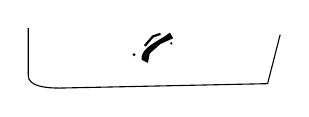
\begin{tikzpicture}[x=1cm,y=1cm,scale=.8]
\draw (0,.9)--(0,.15)..controls(0,-.03)and(.3,-.05)..(.5,-.05)--(3.8,.02)--(4,.8);
\fill (1.8,.4)..controls(1.78,.55)and(1.96,.65)..(2.15,.76)--(2.25,.83)--(2.3,.74)--(2.1,.65)--(1.93,.5)--(1.9,.35)--cycle;
\draw[line width=.8pt] (1.85,.62)--(1.98,.77)--(2.1,.81);
\fill(1.68,.48)circle(.025);\fill(2.27,.66)circle(.02);
\end{tikzpicture}}

\deleted{\uline{Proposition}}\inserted{Cor. 3} Soient $\deleted{F}G,F$ deux figures. Pour que $\deleted{F}G\subset F$\inserted{ (i.e. $G$ sous figure de $F$)}, il f et s. que $\deleted{F}G$ \uline{compatible} à $F$ (i.e. $\deleted{\unsure{G|F}}F\cup\deleted{F}G$ une figure, soit $\deleted{\unsure{F|G}}H$) et $\deleted{F}G\ll F$, i.e $G\subset\deleted{G'}F'$, $\deleted{\unsure{G|F}}F'$ sub. de $F$.

En effet, par \deleted{\unsure{Cont|Cond|C}} C 4, \deleted{comme}
\diagram{\begin{tikzcd}[ampersand replacement=\&,row sep=.15em,column sep=.25em]
F \& \subset \& H=F\cup G \\
F'\arrow[u,Rightarrow,"\text{subd.}"] \& {} \& {}\\
\tikz[baseline=-.5ex]\node[rotate=90,inner sep=0pt] {$\subset$}; \& {} \& {}\\
\deleted{\unsure{F|G}}G \& {} \& {}
\end{tikzcd}}
% The following calculation is written immediately to the right of the diagram.
\[
G\subset \underset{\deleted{\unsure{F'\cap H|G'\cap H}}}{\deleted{G'}F'\cap H}\ \deleted{\unsure{\subset G'\cap H|\subset F'\cap H}}\ \underset{\mathrm C\,4}{\mathrel{\tikz[baseline=-.35ex]\draw[line cap=round] (.35,.16) .. controls (.12,.18) and (.02,.08) .. (0,0) -- (1.18,0);}}\ F
\]
donc $G\subset F$.

En particulier, on trouve :
% slanted
\margin{C'est la partie sérieuse de C 4 \(\left(\vphantom{\dfrac{1}{1}}\right.\)}
\[
\text{Si } X\in M,\ F\in\mathcal F,\ \text{alors}\quad X\in F\ \Longleftrightarrow\
\left\{\begin{aligned}
&X\ \text{comp. à }F\\
&X\ \text{raffine }F
\end{aligned}\right.
\]
donc
\[
\text{Si } X,Y\in M,\ \text{alors}\quad X\leq Y\ \Longleftrightarrow\
\left\{\begin{aligned}
&X\ \text{comp. à }Y\\
&X\ \deleted{\text{raffine}}\ll Y
\end{aligned}\right.
\]

% slanted
\margin{\uline{NB} $F$ et $G$ disj. ssi $X\in F,\ Y\in G\Rightarrow X$ et $Y$ disj.$^{\mathrm{ts}}$ (i.e. ou non compatibles, \unsure{ou} $X$ et $Y$ \unsure{elt|et} \uuline{distincts})}

\deleted{\uline{\unsure{C 5|C 2}}} $F,G\in\mathcal F$ sont dites \uline{disjointes} si elles sont compatibles (i.e $F\cup G\in\mathcal F$) et $F\cap G=\varnothing$. On dit que $X,Y$ sont disjointes, ssi $F_X$ et $F_Y$ le sont i.e. $X$ et $Y$ compatibles, et $\nexists Z$ avec $Z\leq X,Y$.

Si $F$ et $G$ sont disjointes, alors pour $F'\subset F,G'\subset G$ sous-figures, elles sont disjointes. De plus ;
